\documentclass[10pt]{beamer}

\usepackage{appendixnumberbeamer}

% \usepackage{beamerposter}

\usepackage{fontspec}

\usepackage{csquotes}
\usepackage[greek,main=brazil]{babel}

\usepackage{linguex}
\usepackage{tikz} %for all basic options
\usepackage{tikz-qtree} %for simple tree syntax
\usepackage{booktabs}
\usepackage[normalem]{ulem}
\usepackage{hyphenat}
\usepackage{multirow}
\usepackage{pgfplots}
\usepackage{paralist}

\usetheme[
	progressbar=foot,
	sectionpage=progressbar,
	numbering=fraction]{metropolis}

\newcommand\Wider[2][4em]{%
	\makebox[\linewidth][c]{%
		\begin{minipage}{\dimexpr\textwidth+#1\relax}
			\raggedright#2
		\end{minipage}%
	}%
}

\title{Ser necessário fazer e ordenar fazer}
\subtitle{Classificadores gêneros literários por meio de classes verbais do grego}
\author{Caio Borges Aguida Geraldes\newline \texttt{caio.geraldes@usp.br}\vspace{5pt}}
\institute{FFLCH-USP\\
\includegraphics[height=0.40cm]{logo-fapesp.png}}

\setsansfont{Gentium Plus}
\setmonofont[Scale=0.75]{Noto Sans Mono}

\usepackage[
	backend=biber,
	style=authoryear,
	autolang=hyphen,
]{biblatex}
\addbibresource{biblio.bib}

\definecolor{obl}{RGB}{41,5,195}
\definecolor{teste}{RGB}{46,139,87}
\definecolor{verb}{RGB}{255, 0, 0}
\definecolor{acc}{RGB}{11,92,16}
\definecolor{atr}{RGB}{128,0,128}
\newcommand{\Vum}[1]{#1}
\newcommand{\Vdois}[1]{#1}
\newcommand{\Obl}[1]{\textcolor{obl}{\uline{#1}}}
\newcommand{\XAcu}[1]{\textcolor{acc}{\uline{#1}}}
\newcommand{\XObl}[1]{\textcolor{atr}{\uline{#1}}}
\newcommand{\vum}[1]{\textbf{#1}}
\newcommand{\vdois}[1]{\textbf{#1}}
\newcommand{\oobl}[1]{\textbf{#1}}
\newcommand{\xobl}[1]{\textbf{#1}}

\begin{document}

\maketitle

\begin{frame}
	\frametitle{Exemplo}
	\ex.\a.\Vum{συμβουλεύει} \Obl{τῷ Ξενοφῶντι} \XAcu{ἐλθόντα} {εἰς Δελφοὺς} \Vdois{ἀνακοινῶσαι} {τῷ θεῷ} {περὶ τῆς πορείας}. (Xen. Anab. 3.1.5)\vspace{5pt}\\
	Ele aconselha Xenofonte a ir a Delfos perguntar sobre a viagem.\vspace{10pt}
	\b.ἀφῆκέ \Obl{μοι} \XObl{ἐλθόντι} πρὸς ὑμᾶς λέγειν τἀληθῆ. (Xen. Hell. 6.1.13)\vspace{5pt}\\
	Ele me permitiu ir frente a vós dizer a verdade.


\end{frame}

\begin{frame}
	\frametitle{Classes de verbo que permitem atração}
	\begin{compactenum}
		\item verbos pessoais com a semântica de `\emph{ordenar}\slash{}\emph{pedir} \slash{}\emph{aconselhar}\slash{}etc. [a alguém] [fazer algo]' (e.g. παραγγέλλω, δέομαι e συμβουλεύω);
		\item a forma impessoal do verbo δοκέω `parecer bom [a alguém] [fazer algo]';
		\item verbos impessoais que denotam a possibilidade ou necessidade da ação infinitiva `ser possível\slash{}suficiente\slash{}necessário [a alguém] [fazer algo]' (e.g. ἔξεστι, ἐξαρκεῖ e προσήκει).
	\end{compactenum}
\end{frame}

\begin{frame}
	\frametitle{Autoria, gênero e atração}
	\begin{table}[!h]
		\begin{center}
			\begin{tabular}[t]{lrr}
				\toprule
				                               & Sem atração  & Com atração  \\
				\midrule
				Platão                         & 13 (48.1\%)  & 14 (51.8\%)  \\
				Xenofonte (diálogo filosófico) & 4   (40.0\%) & 6 (60.0\%)   \\
				\midrule
				Diálogo filosófico (Total)     & 17 (45.9\%)  & 20  (54.1\%) \\
				\midrule
				\midrule
				Xenofonte (prosa histórica)    & 29 (64.5\%)  & 16  (35.5\%) \\
				Heródoto                       & 35 (92.1\%)  & 3   (7.8\%)  \\
				\midrule
				Prosa histórica (Total)        & 64 (77.1\%)  & 19  (22.8\%) \\
				\bottomrule
			\end{tabular}
		\end{center}
	\end{table}
\end{frame}

\begin{frame}
	\frametitle{Modelo resultante}
	\begin{table}[!ht]
		\centering
		\begin{tabular}{lllll}
			\toprule
			{}             & precisão & cobertura & $F_1$ & suporte \\
			\midrule
			historiografia & 0.81     & 0.76      & 0.79  & 4696    \\
			filosofia      & 0.79     & 0.84      & 0.82  & 5136    \\
			\midrule
			acurácia       &          &           & 0.80  & 9832    \\
			macro avg      & 0.80     & 0.80      & 0.80  & 9832    \\
			weighted avg   & 0.80     & 0.80      & 0.80  & 9832    \\
			\bottomrule
		\end{tabular}
	\end{table}
\end{frame}

\begin{frame}
	\frametitle{Modelo resultante}
	\begin{figure}[!ht]
		\begin{center}
			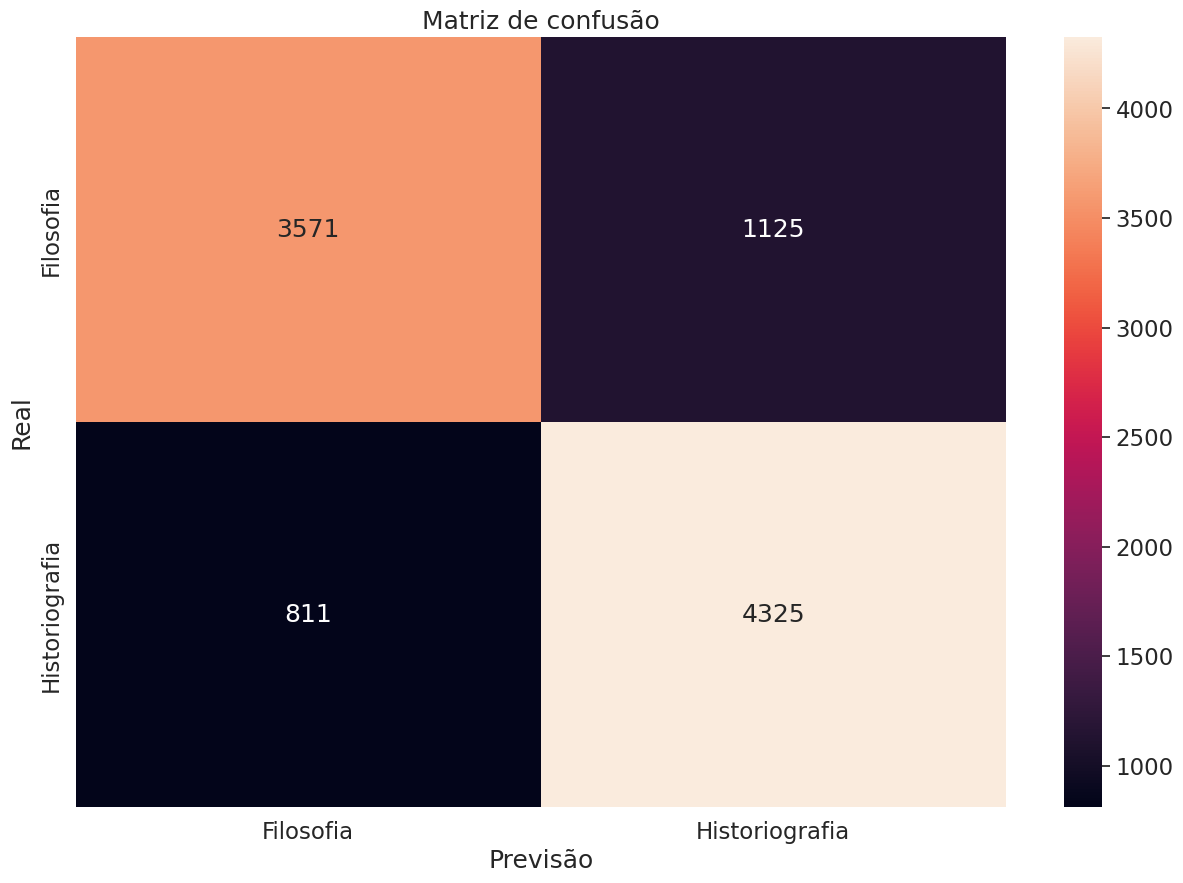
\includegraphics[width=1\linewidth]{./figs/confusao.png}
		\end{center}
	\end{figure}
\end{frame}

\begin{frame}
	\Wider{
		\begin{figure}[!ht]
			\begin{center}
				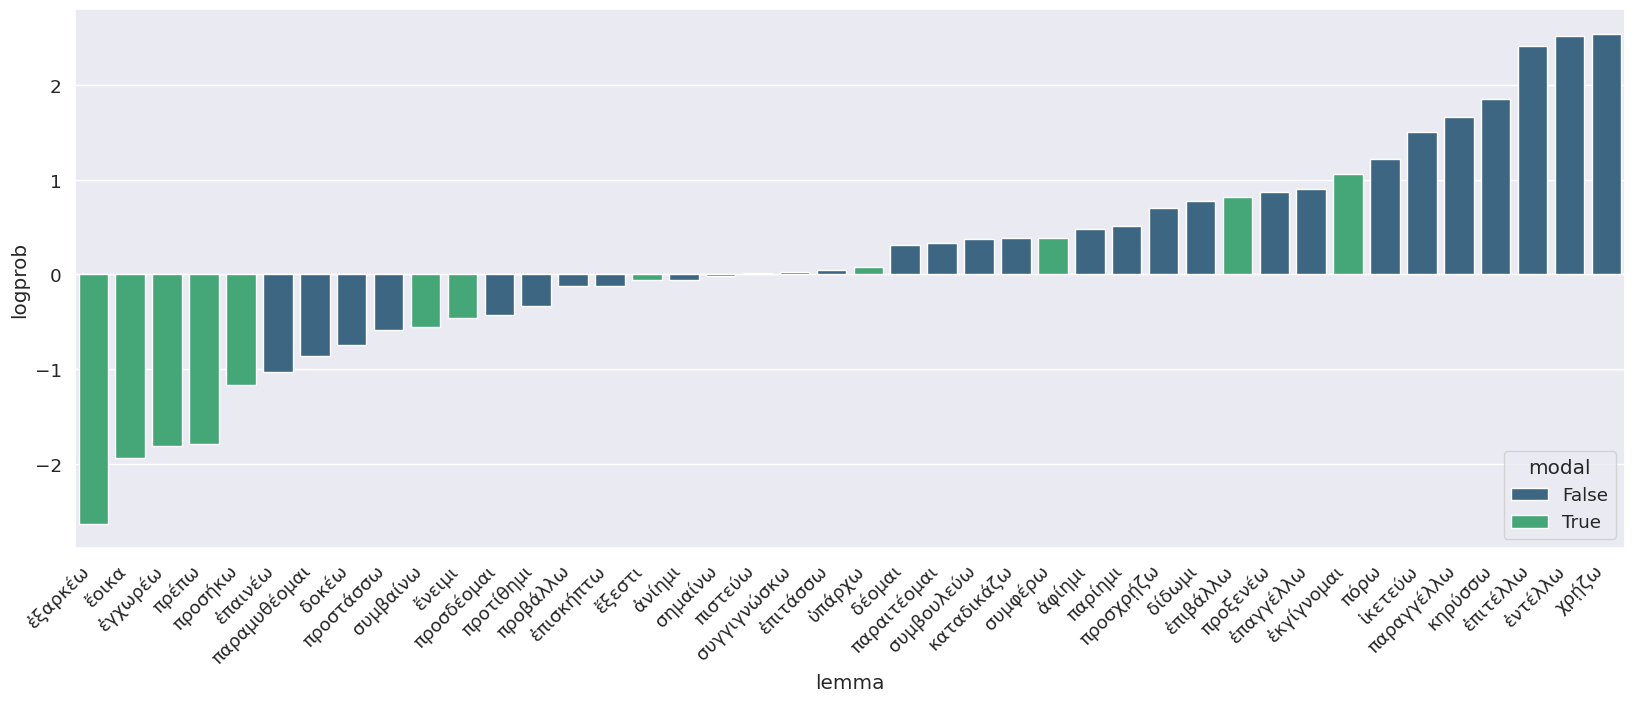
\includegraphics[width=1\linewidth]{./figs/diff2.png}
			\end{center}
		\end{figure}
	}
\end{frame}


\begin{frame}[standout]
	\normalsize
	Contato:\\
	\texttt{caio.geraldes@usp.com}

	Dados e código disponíveis em:\\
	\texttt{github.com/caiogeraldes/2023sbec}
\end{frame}


\end{document}
